

\documentclass[preprint,12pt]{elsarticle}

\usepackage[spanish]{babel}
\usepackage{amssymb}
\usepackage{graphicx}
\usepackage{lineno}
\usepackage[utf8]{inputenc}
\usepackage{url}
\usepackage{natbib} 
\usepackage{amsmath} 
\usepackage{amssymb} 

\begin{document}
	
	\begin{frontmatter}

		\title{\huge Gestores de BD NoSQL}
		
		\author{Aponte Roldán, Sigfredo              		(2016054468))}
		\author{Gonzales Cave, Angel Gabriel              	(2017057861))} %%cambiar
		\author{Pacora Silva, Jorge Carlos         		(2013000725))} %%cambiar
		\author{Quispe Mamani, José Luis             		())} %%cambiar 
		\address{Tacna, Perú}
		
%% ABSTRACT --------------------------------------------------------------------------------------------------------------------
\begin{abstract}
		
MongoDB stores data in flexible documents similar to JSON, so the fields may vary between documents and the data structure may change over time.

The document model is assigned to the objects in the code of your application to facilitate the work with the data

Ad hoc queries, real-time indexing and aggregation offer powerful ways to access and analyze data

MongoDB is a database distributed at its core, so high availability, horizontal scalability and geographic distribution are integrated and easy to use.

MongoDB is free to use. Versions released before October 16, 2018 are published under the AGPL license. All versions after October 16, 2018, including patches released for earlier versions, are published under Public Server License (SSPL) v1.

\end{abstract}

%% ----------------------------------------------------------------------------------------------------------------------------------

	\end{frontmatter}

%% RESUMEN ---------------------------------------------------------------------------------------------------------------------

\section{Resumen}
MongoDB almacena datos en documentos flexibles similares a JSON, por lo que los campos pueden variar entre documentos y la estructura de datos puede cambiarse con el tiempo

El modelo de documento se asigna a los objetos en el código de su aplicación para facilitar el trabajo con los datos

Las consultas ad hoc, la indexación y la agregación en tiempo real ofrecen maneras potentes de acceder a los datos y analizarlos

MongoDB es una base de datos distribuida en su núcleo, por lo que la alta disponibilidad, la escalabilidad horizontal y la distribución geográfica están integradas y son fáciles de usar

MongoDB es de uso gratuito. Las versiones lanzadas antes del 16 de octubre de 2018 se publican bajo licencia AGPL. Todas las versiones posteriores al 16 de octubre de 2018, incluidos los parches lanzados para versiones anteriores, se publican bajo Licencia pública del lado del servidor (SSPL) v1.


%% ----------------------------------------------------------------------------------------------------------------------------------


%% INTRODUCION ----------------------------------------------------------------------------------------------------------------

\section{Introducción} 
Si tuviésemos que explicar qué es MongoDB podríamos decir que es una base de datos opensource NOSQL basada en documentos desarrollada por la gente de 10gen. Aunque una vez que cogió auge la base de datosMongoDB pasaron a llamarse con el mismo nombre y ahora la empresa y el producto se llaman MongoDB. El nombre de MongoDB proviene de “humongous”, que significa enorme en inglés. MongoDB es una base de datos NOSQL, opensource, escrita en C++, escalable y de alto rendimiento.

MongoDB y los documentos
El elemento principal de MongoDB es como almacena la información. MongoDB almacena toda la información en documentos JSON.

El almacenar la información en documentos JSON permite a MongoDB tener independencia del schema de almacenamiento, es decir, pueden existir más o menos campos en el documento dentro de una misma colección de documentos. Una de las cosas importantes de los documentos es que estos van tipados. Además los documentos nos permiten nuevas estructuras como arrays o subdocumentos que permitirán que de una sola consulta se recupere toda la información y evite así la necesidad de ejecutar consultas de tipo join.

Principales características de MongoDB
Aunque en los siguientes capítulos iremos viendo en detalle todas las funcionalidades de MongoDB, podríamos decir que las principales características de MongoDB son:

Alto rendimiento
El alto rendimiento para la persistencia en MongoDB se basa en dos puntos: La posibilidad de tener documentos con la información anidada, evitando, de esta forma, un número elevado de operaciones de I/O. Y el soporte de índices y la posibilidad de crear índices sobre arrays y subdocumentos.

Alta disponibilidad
MongoDB proporciona alta disponibilidad mediante la réplica automática conocida como replica set, la cual proporciona redundancia de datos y failover automático, es decir, la transferencia automática a un nuevo nodo cuando se encuentra un fallo en uno de los nodos.

Escalado Automático
MongoDB nos ofrece un escalado horizontal. Para ello el sistema de sharding nos permite distribuir información por diferentes cluster de máquinas.

%% ----------------------------------------------------------------------------------------------------------------------------------


%% MARCO TEÓRICO ------------------------------------------------------------------------------------------------------------

\section{Marco Teórico}

%% PRIMERA SUBSECCION 

\subsection {\textbf{Base de datos NoSQL orientadas a Documentos}}
Una base de datos orientada a documentos está diseñada para gestionar información orientada a documentos o datos semiestructurados. Tienen un grado de complejidad y flexibilidad superior a las bases de datos clave – valor. \newline
A diferencia de las conocidas bases de datos relacionales con su definición de “tabla”, los sistemas documentales están diseñados entorno a la definición abstracta de un “documento”. Un documento es la unidad principal de almacenamiento de este tipo de base de datos, y toda la información que aquí se almacena, se hace en formato de documento. \newline

Este tipo de Base de Datos NoSQL almacena la información como un documento, generalmente utilizando para ello una estructura simple como JSON o XML y donde se utiliza una clave única para cada registro. Este tipo de implementación permite, además de realizar búsquedas por clave – valor, realizar consultas más avanzadas sobre el contenido del documento.
\cite{BDnoSQLMongodb}
\subsubsection{\textbf{Ventajas}}
\begin{itemize}

\item Almacenar y recuperar todos los datos relacionados como una sola unidad puede entregar ventajas enormes en el rendimiento y la escalabilidad.
\item Los gestores no tienen que hacer operaciones complejas como las uniones para encontrar los datos que normalmente están relacionados, ya que todo se encuentra en un mismo lugar.
\end{itemize}

\cite{BDnoSQLMongodb}
\subsection {\textbf{MongoDB}}
MongoDB es una base de datos NoSQL Open Source orientada a documentos y ha sido diseñada con la idea de que fuera fácil tanto desarrollar para ella como de ser administrada. Un documento es una estructura de datos compuesta de pares de campos y valores. Además, estos objetos son muy similares a lo que serían objetos en notación JSON. \newline
Utilizar documentos tiene ciertas ventajas:
\begin{itemize}

\item Los documentos son tipos de datos nativos en muchos lenguajes de programación.
\item Los documentos embebidos y los arrays minimizan la necesidad de realizar joins muy pesados.
\item Tener un esquema dinámico es la base del polimorfismo.

\end{itemize}
 \cite{MongoDB}
\subsubsection{\textbf{Características generales}}
\begin{itemize}
\item 
\textbf{Indexado}\newline
MongoDB soporta índices secundarios, permitiendo una buena aceleración en muchas querys, pudiendo indexar cualquier campo de la base de datos.
\item 
\textbf{Agregación}\newline
MongoDB viene con muchas funciones predefinidas que facilitan en gran medida el tratamiento de las colecciones almacenadas.
\item
\textbf{Replicación y Balanceo de Carga}\newline
MongoDB utiliza un sistema de replicación empleando la arquitectura maestro – esclavo con el resto de máquinas. Además, hace uso de un tipo de particionado horizontal llamado sharding. Estas dos herramientas de escalado hacen de mongo una herramienta poderosa cuando se trata de crecer mucho en poco tiempo.

Mientras que la replicación busca realizar copias de los datos, repartirlos por nuevos hosts, permitiendo ofrecer alta disponibilidad, balanceo de carga y copias automáticas de seguridad, el sharding busca particionar esas tablas que, previsiblemente, se van haciendo más grandes y cada vez son más costosas de replicar.
\end{itemize}
 \cite{MongoDB}

\begin{figure}[htb]
	\begin{center}
		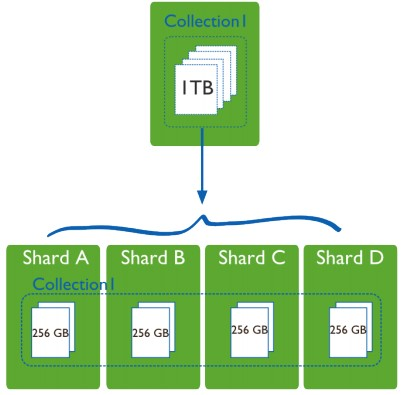
\includegraphics[width=6cm]{./IMAGENES/img01} %%EJEMPLO PARA INCLUIR IMAGEN
	\end{center}
\end{figure}

\subsubsection{\textbf{Modelo de datos}}

MongoDB es un tipo de base de datos de esquema flexible. Esto significa que ha de ser el usuario el que el que determina y declara el esquema de cada una de las tablas justo en el momento de realizar las inserciones.
Por un lado se tiene la flexibilidad de añadir campos cuando son necesarios sin haberlos tenido que haberlos definido de antemano, o obviar algunos en los casos en los que no sean necesarios, pero a la vez se obliga al programador a ser mucho más metódico en su trabajo, puesto que el sistema no avisará de un posible error o despiste en el código.

\subsubsection{\textbf{BSON}}

BSON es un formato binario que se utiliza para almacenar la información en MongoDB. BSON es la codificación binaria del formato JSON. Esta codificación ha sido elegida porque presenta ciertas ventajas a la hora de almacenar los datos, como la eficiencia o la compresión.
Básicamente BSON y JSON son los formatos con los que trabaja MongoDB: JSON es el formato con el que se presenta la información a los usuarios y a las aplicaciones y BSON el formato que utiliza MongoDB de forma interna.

\subsubsection{\textbf{Estructura del documento}}

El reto principal que tienen los documentos como objetos en MongoDB es el de realizar un buen diseño de los mismos para que sean capaces de representar lo más ampliamente el mundo real. Para ello existen 2 herramientas que permiten a las aplicaciones representar las relaciones entre los datos: las referencias y los datos embebidos. Una de las decisiones a tomar a la hora de implementar una aplicación que utilice MongoDB como capa de backend de aplicación es la de referenciar o embeber los documentos que se necesite.

\subsubsection{\textbf{Referencias}}
Las referencias almacenan relaciones entre los datos mediante enlaces entre documentos.
Los modelos de datos normalizados utilizan relaciones referenciales entre los documentos. Se usarán modelos de datos normalizados cuando:

\begin{itemize}

\item Embeber documentos produzca una duplicación de la información y los costes de mantenimiento sean mayores que las ganancias en lecturas.
\item Sea necesario representar un modelo “varios a varios” con cierta complejidad.
\item Para modelar conjuntos de datos de mucho tamaño.

\end{itemize}

\begin{figure}[htb]
	\begin{center}
		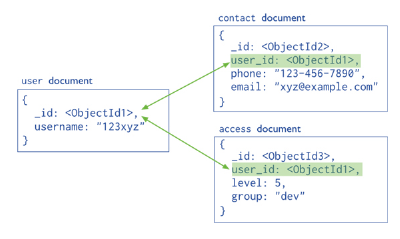
\includegraphics[width=10cm]{./IMAGENES/img02.png} %%EJEMPLO PARA INCLUIR IMAGEN
	\end{center}
\end{figure}
 \cite{MongoDB}


\subsubsection{\textbf{Datos embebidos}}
Los documentos embebidos representan relaciones entre los datos almacenando la información relacionada bajo el mismo documento. Los documentos permiten embeber estructuras documentales como subdocumentos dentro de un campo o de un array.
En general, se utilizarán modelos embebidos cuando:
\begin{itemize}

\item Existan relaciones contenidas entre dos entidades. Estos es, que dos entidades independientes sean habitualmente accedidas a través de sólo una de ellas. Por ejemplo, Persona y Dirección. Cuando únicamente se permitan búsquedas por persona para obtener su dirección. En ese caso, es preferible tener el objeto Dirección embebido dentro del de Persona.
\item Cuando exista una relación “uno a varios” entre entidades. En este caso, la parte de “varios” suele ir embebida dentro de la de “uno”. Los motivos son similares al anterior caso.
\item En general, en ambos se trata de minimizar en la medida de los posible las operaciones de la base de datos. Embebiendo la información se consigue leer o escribir todos los datos simultáneamente y de forma secuencial.
\end{itemize}
 \cite{MongoDB}
\begin{figure}[htb]
	\begin{center}
		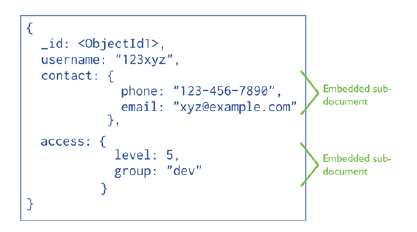
\includegraphics[width=10cm]{./IMAGENES/img03.png} %%EJEMPLO PARA INCLUIR IMAGEN
	\end{center}
\end{figure}





%% ----------------------------------------------------------------------------------------------------------------------------------


%% ANÁLISIS ( APLICACIÓN ) ---------------------------------------------------------------------------------------------------

\section{Análisis (Aplicación)}

\subsection {\textbf{Mongo DB}}
Una de las razones principales porr la que los desarroladores usan MongoDB es debido a su modelo de datos intuitivo. MongoDB almacena su información en documentos en lugar de filas. ¿Qué es un documento? Aqui hay un ejemplo:
\subsubsection{\textbf{Esquema Básico}}
Los productos y las categorías son los pilares de cualquier sitio de comercio electrónico. Los productos, en un modelo RDBMS(Sistema de gestión de bases de datos relacionales) normalizado, tienden a requerir una gran cantidad de tablas. Hay una mesa para
información básica del producto, como el nombre y el código, pero habrá otras tablas para
Relacionar la información de envío y los historiales de precios. Este esquema multitarea será facilitado por la capacidad del RDBMS para unir tablas.
 Modelar un producto en MongoDB debería ser menos complicado. Debido a que las colecciones no aplican un esquema, cualquier documento del producto tendrá espacio para cualquier
atributos dinámicos que necesita el producto. Mediante el uso de matrices en su documento, puede
normalmente condensa una representación RDBMS multitable en una sola colección MongoDB.
\begin{figure}[htb]
	\begin{center}
		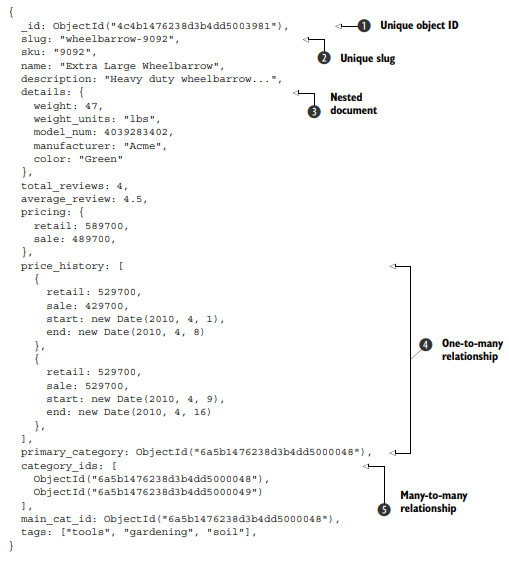
\includegraphics[width=10cm]{./IMAGENES/mongodb1} %%EJEMPLO PARA INCLUIR IMAGEN
	\end{center}
\end{figure}
Más concretamente, la imagen muestra un producto de muestra de una tienda de jardinería. Es recomendable asignar este documento a una variable antes de insertarlo en la base de datos utilizando
"db.products.insert (yourVariable)" para poder ejecutar las consultas discutidas durante las
siguientes varias páginas.

\cite{Nosql}

\subsubsection{\textbf{Usuarios y ordenes}}
Si observa cómo modela los usuarios y los pedidos, verá otra relación común: uno a muchos. Es decir, cada usuario tiene muchos pedidos. En un RDBMS(Sistema de gestión de bases de datos relacionales), usaría una clave foránea en su tabla de pedidos; aquí, la convención es similar.
\begin{figure}[htb]
	\begin{center}
		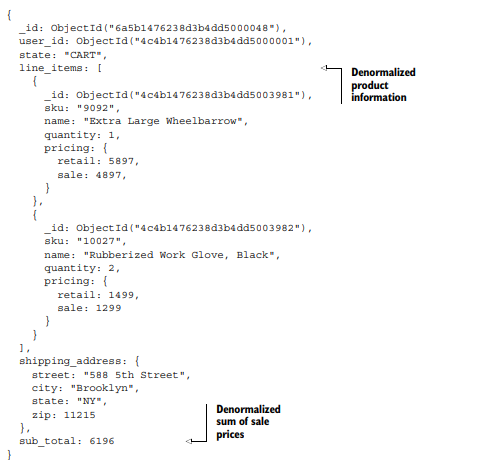
\includegraphics[width=10cm]{./IMAGENES/mongodb2} %%EJEMPLO PARA INCLUIR IMAGEN
	\end{center}
\end{figure}
\subsubsection{\textbf{Manejando Bases de Datos}}
No existe una fomra explicita de vrear una base de datos en MongoDB. En cambio, una base de datos se crea automaticamente una vez que escribe en una coleecion en esa base de datos. A continuacion veremos un ejemplo:
\begin{figure}[htb]
	\begin{center}
		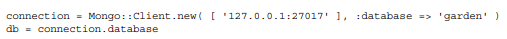
\includegraphics[width=15cm]{./IMAGENES/mongodb3} %%EJEMPLO PARA INCLUIR IMAGEN
	\end{center}
\end{figure}

Suponiendo que la base de datos no existe, la base de datos no se a creado en el disco luego de haber ejecutado el codigo mencionado. Todo lo que se ha hecho es instanciar una instancia de la clase Mongo::DB, que representa una base de datos de MongoDB. Para crear nuestra base de datos se debera ejecutar el código siguiente:
\begin{figure}[htb]
	\begin{center}
		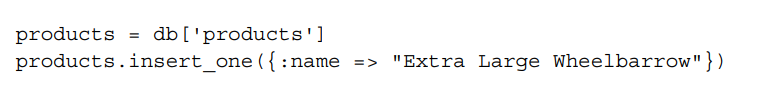
\includegraphics[width=15cm]{./IMAGENES/mongodb4} %%EJEMPLO PARA INCLUIR IMAGEN
	\end{center}
\end{figure}
\cite{Raul2014}
%% ----------------------------------------------------------------------------------------------------------------------------------


%% CONCLUSIONES ---------------------------------------------------------------------------------------------------------------

\section{Conclusiones}

\begin{itemize}

\item Conclusion 1 : \\ Este artículo describe las limitaciones de las bases de datos tradicionales.
y las ventajas de la base de datos NO SQL, análisis, objetivo de sus fortalezas
y debilidades respectivamente, lo que ayudará al usuario a elegir
entre una base de datos NO SQL y una base de datos tradicional.

\item Conclusion 2 : \\ Son muchos los casos en el que se requiere realizar un previo análisis sobre que tipo de base de datos NoSQL es la mejor opción, ya que los diferentes tipos de base de datos NoSQL están orientados a brindar diferentes soluciones dependiendo del caso o aplicativo que deseamos implementar.


\end{itemize}

%% ----------------------------------------------------------------------------------------------------------------------------------

%%  REFERENCIAS BIBLIOGRÁFICAS ------------------------------------------------------------------------------------------
	
	\newpage
	
	\bibliographystyle{apalike} 	%ESTILO
	\bibliography{BIBLIOGRAFIA}	 
	
	
\end{document}
